\documentclass[
11pt, % The default document font size, options: 10pt, 11pt, 12pt
codirector, % Uncomment to add a codirector to the title page
]{charter} 

% El títulos de la memoria, se usa en la carátula y se puede usar el cualquier lugar del documento con el comando \ttitle
\titulo{Título del proyecto} 

% Nombre del posgrado, se usa en la carátula y se puede usar el cualquier lugar del documento con el comando \degreename
\posgrado{Carrera de Especialización en Sistemas Embebidos} 
%\posgrado{Carrera de Especialización en Internet de las Cosas} 
%\posgrado{Carrera de Especialización en Intelegencia Artificial}
%\posgrado{Maestría en Sistemas Embebidos} 
%\posgrado{Maestría en Internet de las cosas}

% Tu nombre, se puede usar el cualquier lugar del documento con el comando \authorname
\autor{SISE-RS versión B} 

% El nombre del director y co-director, se puede usar el cualquier lugar del documento con el comando \supname y \cosupname y \pertesupname y \pertecosupname
\director{Nombre del Director}
\pertenenciaDirector{pertenencia} 
% FIXME:NO IMPLEMENTADO EL CODIRECTOR ni su pertenencia
\codirector{John Doe} % para que aparezca en la portada se debe descomentar la opción codirector en el documentclass
\pertenenciaCoDirector{FIUBA}

% Nombre del cliente, quien va a aprobar los resultados del proyecto, se puede usar con el comando \clientename y \empclientename
\cliente{Nombre del cliente}
\empresaCliente{Empresa del cliente}

% Nombre y pertenencia de los jurados, se pueden usar el cualquier lugar del documento con el comando \jurunoname, \jurdosname y \jurtresname y \perteunoname, \pertedosname y \pertetresname.
\juradoUno{Nombre y Apellido (1)}
\pertenenciaJurUno{pertenencia (1)} 
\juradoDos{Nombre y Apellido (2)}
\pertenenciaJurDos{pertenencia (2)}
\juradoTres{Nombre y Apellido (3)}
\pertenenciaJurTres{pertenencia (3)}
 
\fechaINICIO{30 de abril de 2021}		%Fecha de inicio de la cursada de GdP \fechaInicioName
\fechaFINALPlan{18 de junio de 2021} 	%Fecha de final de cursada de GdP
\fechaFINALTrabajo{15 de mayo de 2022}	%Fecha de defensa pública del trabajo final


\begin{document}

\maketitle
\thispagestyle{empty}
\pagebreak


\thispagestyle{empty}
{\setlength{\parskip}{0pt}
\tableofcontents{}
}
\pagebreak


\section*{Registros de cambios}
\label{sec:registro}

\begin{table}[ht]
\label{tab:registro}
\centering
\begin{tabularx}{\linewidth}{@{}|c|X|c|@{}}
\hline
\rowcolor[HTML]{C0C0C0} 
Revisión & \multicolumn{1}{c|}{\cellcolor[HTML]{C0C0C0}Detalles de los cambios realizados} & Fecha      \\ \hline
A & Creación del documento & 27/06/2021 \\ \hline
B & Se cambia el formato a pedido de la cátedra en la cursada del día 28/06/2021. \newline
	Se incorporan cambios según la reunión del día 29/06/2021. & 29/06/2021 \\ \hline
%2 & Se completa hasta el punto 7 inclusive
%		  Se puede agregar algo más \newline
%		  En distintas líneas \newline
%		  Así                                                    & dd/mm/aaaa \\ \hline
%3      & Se completa hasta el punto 11 inclusive                & dd/mm/aaaa \\ \hline
%4      & Se completa el plan	                                 & dd/mm/aaaa \\ \hline
\end{tabularx}
\end{table}

\pagebreak

\section{1. Introducción}
\label{sec:introduccion}

\subsection{Propósito}

Este documento representa una especificación de requerimientos de software para un sistema de inyección de soft-errors. Está dirigido a las personas que se ocupen de las siguientes tareas:
\begin{itemize}
	\item análisis
	\item diseño
	\item implementación
	\item pruebas
\end{itemize}

\subsection{Ámbito del sistema}

El nombre del sistema será SISE y permitirá inyectar errores en todos los registros accesibles del microcontrolador SAMV71. Su función será evaluar las técnicas de mitigación de soft-errors en funciones a ser utilizadas en misiones espaciales.

El beneficio que se espera obtener es utilizar componentes que no fueron sometidos a un proceso de calificación. Los clasificados como alternativos.

\subsection{Definiciones, acrónimos y abreviaturas}

\subsection{Referencias}

INVAP - Propuesta de tesis: sistema de inyección de soft-errors.

\subsection{Visión general del documento}

Este documento se realizó según lo especificado en el estándar IEEE Std. 830-1998.

\section{2. Descripción general}
\label{sec:descripcion}

\subsection{Perspectiva del producto}

El software aquí especificado es independiente de otros sistemas y no tiene relación con otros productos.
En la figura \ref{fig:esqGral} se puede observar el campo de acción del software propuesto.

\begin{figure}[h]
	\centering
	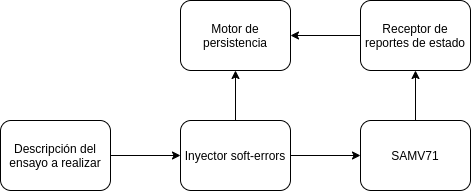
\includegraphics[width=0.7\textwidth]{./Figuras/SISE.png}
	\caption{esquema general del sistema.}
	\label{fig:esqGral}
\end{figure}

El inyector de soft-errors deberá modificar los registros del microcontrolador SAMV71 según lo dispuesto en la descripción del ensayo.
En simultaneo, se debe persistir la modificación realizada.
Luego, se debe reportar el estado de funcionamiento del microcontrolador.
Finalmente, los reportes deben ser persistidos para su análisis.

\subsection{Funciones del producto}

El software aquí especificado brindará las siguientes funcionalidades:

\begin{itemize}
	\item Inyección de errores en todos los registros accesibles del microcontrolador SAMV71.
	\item Monitoreo del estado de funcionamiento del microcontrolador SAMV71.
	\item Persistencia de los soft-errors inyectados.
	\item Persistencia de los informes de estado de funcionamiento.
	\item Permitir escribir ensayos de evaluación.
	\item Presentación de resultados en histogramas que permitan un análisis estadístico.
\end{itemize}

\subsection{Características de los usuarios}

Los usuarios finales de este producto son ingenieros de desarrollo del INVAP.

\subsection{Restricciones}

Las restricciones del desarrollo del sistema son las siguientes:

\begin{itemize}
	\item Utilización de repositorio con control de versiones Gitlab.
	\item Documentación del código con Doxygen.
	\item Utilización exclusiva del lenguaje de programación Python.
\end{itemize}

\subsection{Suposiciones y dependencias}

La suposición principal es que se tendrá acceso irrestricto al microcontrolador SAMV71.

\subsection{Requisitos futuros}

N/A


\section{3. Requisitos específicos}
\label{sec:requisitos}


\subsection{Interfaces externas}

\begin{itemize}
	\item El software deberá comunicarse por USB con el debugger [SISE-RS-0001-REQ0001].
	\item El software deberá comunicarse por protocolo SERIAL con el microcontrolador SAMV71 [SISE-RS-0001-REQ0002].
\end{itemize}

\subsection{Funciones}

\begin{enumerate}
	\item Inyección de soft-errors:
	\begin{itemize}
		\item Deberá realizar escrituras de 32 bits en la memoria ram [SISE-RS-0001-REQ0003].
		\item Deberá realizar bit-flips en la memoria ram [SISE-RS-0001-REQ0004].
		\item Deberá realizar escrituras en los registros internos respetando su tamaño en bits [SISE-RS-0001-REQ0005].
		\item Deberá realizar bit-flips en los registros internos respetando su tamaño en bits [SISE-RS-0001-REQ0006].
	\end{itemize}
	\item Recepción de reportes:
	\begin{itemize}
		\item Deberá recibir los reportes de estado [SISE-RS-0001-REQ0007].
		\item Deberá relacionar los reportes de estado con la última inyección de soft-error introducida [SISE-RS-0001-REQ0008].
	\end{itemize}
	\item Almacenamiento de reportes:
	\begin{itemize}
		\item Deberá indicar el tiempo transcurrido desde la inyección de soft-error que la precede [SISE-RS-0001-REQ0009].
		\item Deberá generar histogramas para su análisis estadístico [SISE-RS-0001-REQ0010].
	\end{itemize}
\end{enumerate}

\subsection{Requisitos de rendimiento}

El inyector de soft-errors deberá realizar la inserción solicitada en un tiempo menor a 10 ms [SISE-RS-0001-REQ0011].

\subsection{Restricciones de diseño}

Se utilizará el microcontrolador SAMV71 como dispositivo principal [SISE-RS-0001-REQ0012].

\subsection{Atributos del sistema}

\begin{enumerate}
	\item Mantenibilidad:
	\begin{itemize}
		\item El software deberá permitir su modificación para trabajar con otras arquitecturas [SISE-RS-0001-REQ0013].
	\end{itemize}
\end{enumerate}

\subsection{Otros requisitos}

N/A.

\section{4. Apéndices}
\label{sec:apendices}

%\subsection{Formatos de entrada/salida}

%\subsection{Resultados de análisis de costes}

\subsection{Restricciones acerca del lenguaje de programación}

El lenguaje de programación será Python 3 y el código deberá ser documentado según las recomendaciones del manual de usuario de Doxygen.

\end{document}
